\hypertarget{SH__NumericQuestionState_8cpp}{\section{Référence du fichier logic/\-S\-H\-\_\-\-Numeric\-Question\-State.cpp}
\label{SH__NumericQuestionState_8cpp}\index{logic/\-S\-H\-\_\-\-Numeric\-Question\-State.\-cpp@{logic/\-S\-H\-\_\-\-Numeric\-Question\-State.\-cpp}}
}
{\ttfamily \#include \char`\"{}S\-H\-\_\-\-Numeric\-Question\-State.\-h\char`\"{}}\\*
Graphe des dépendances par inclusion de S\-H\-\_\-\-Numeric\-Question\-State.\-cpp\-:
\nopagebreak
\begin{figure}[H]
\begin{center}
\leavevmode
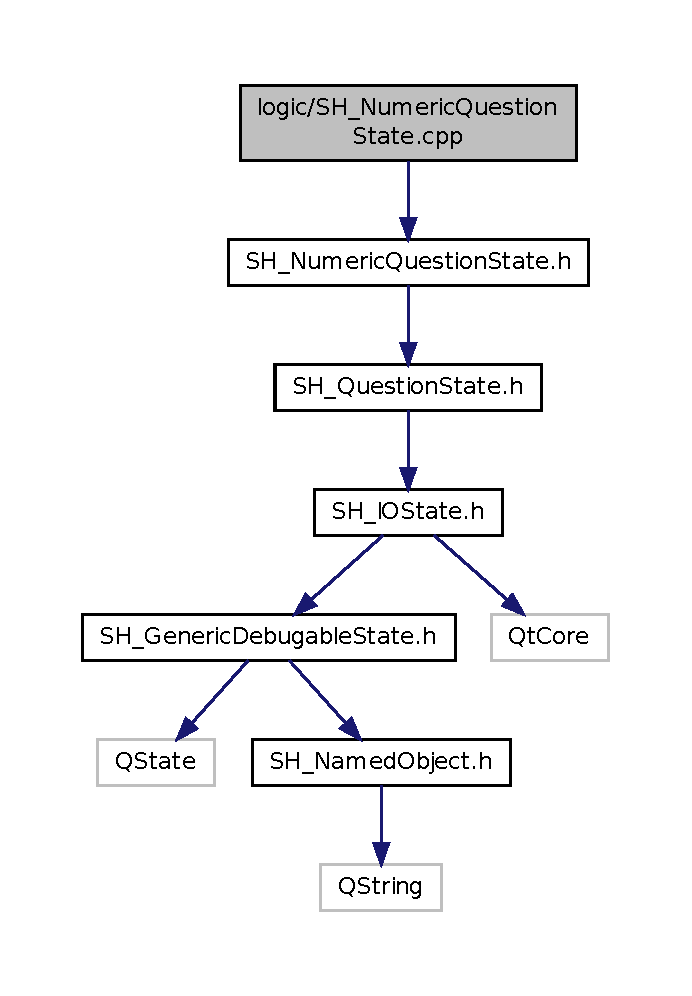
\includegraphics[width=332pt]{SH__NumericQuestionState_8cpp__incl}
\end{center}
\end{figure}
